%!TEX root = ../Technische Dynamik.tex

\tikzstyle{hatch}=[postaction={draw,decorate,decoration={border,angle=-45, amplitude=0.2cm,segment length=1.4mm}}]

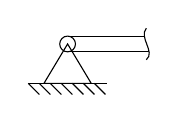
\begin{tikzpicture}[>=latex]

\draw[hatch] (-0.5,0) -- (0.5,0);
\draw[fill=white] (0,0.5) circle (0.1);
\draw (-0.3,0) -- (0.3,0) -- (0,.5) -- cycle;

\draw (0,0.4) -- (1.04,0.4);
\draw (0,0.6) -- (.97,0.6);
\draw (1,0.3) to[in=-130,out=40] (1,0.7);

\end{tikzpicture}